% !TEX program = lualatex
\documentclass[11pt]{article}

% -------- LuaLaTeX : polices et langue --------
\usepackage{fontspec}
\setmainfont{Latin Modern Roman}
\setsansfont{Tex Gyre Heros}
%\renewcommand{\familydefault}{\sfdefault} % force le sans serif par défaut
\usepackage{polyglossia}
\setdefaultlanguage{french}

% -------- Mise en page --------
\usepackage[a4paper,margin=1cm]{geometry}
\usepackage{multicol}
\usepackage{fancyhdr}
\pagestyle{empty}
\usepackage[most]{tcolorbox}

% -------- Mathématiques --------
\usepackage{amsmath,amssymb,mathtools}
\usepackage{icomma}
% \sisetup{locale=FR}

\usepackage{enumitem}
\setlist[itemize]{left=0pt}
\setlist[enumerate]{left=0pt, label=\textbf{\arabic*}.}

\usepackage{ProfCollege}
\usepackage{ProfMaquette}

\usepackage{tabularray}

% -------- Divers --------
\setlength{\parindent}{0pt}

\begin{document}

\begin{multicols}{2}

\begin{Maquette}[Fiche]{Theme=Calcul littéral, Niveau=Quatrième}

\begin{exercice}
    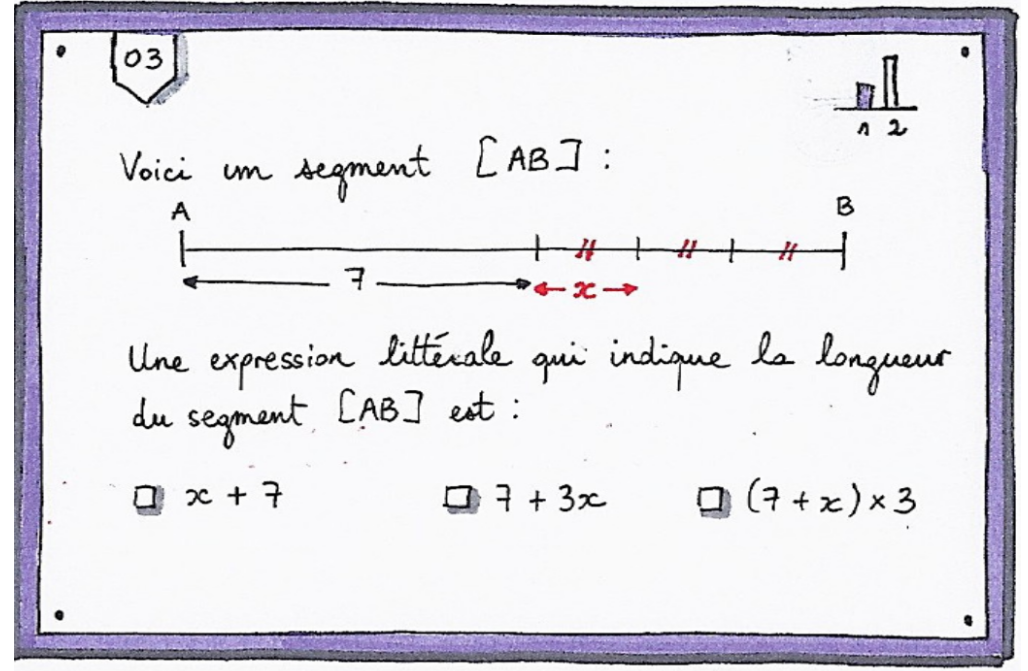
\includegraphics[width=\linewidth]{Images/CalculLitteral1.png}
    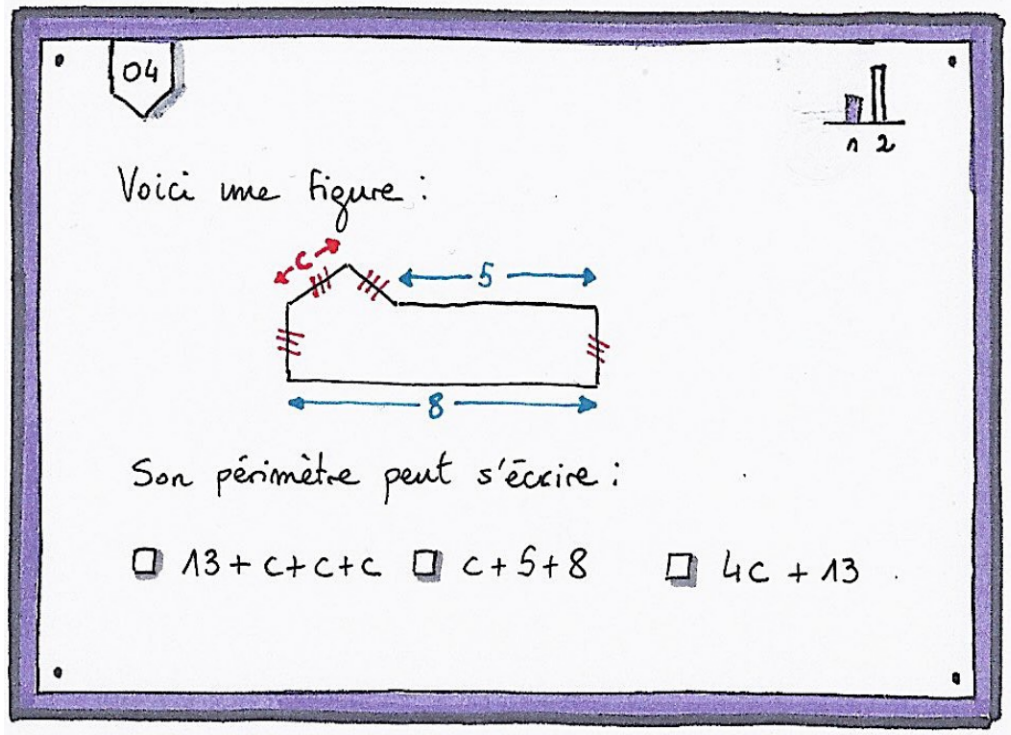
\includegraphics[width=\linewidth]{Images/CalculLitteral2.png}
    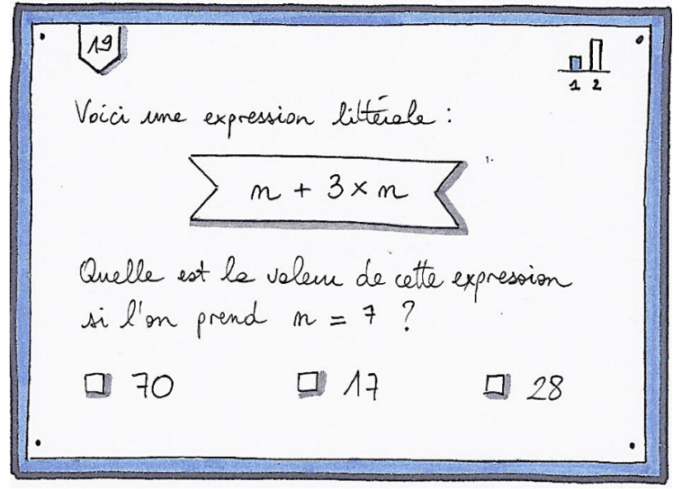
\includegraphics[width=\linewidth]{Images/CalculLitteral3.png}
\end{exercice}

\begin{exercice}
\begin{center}
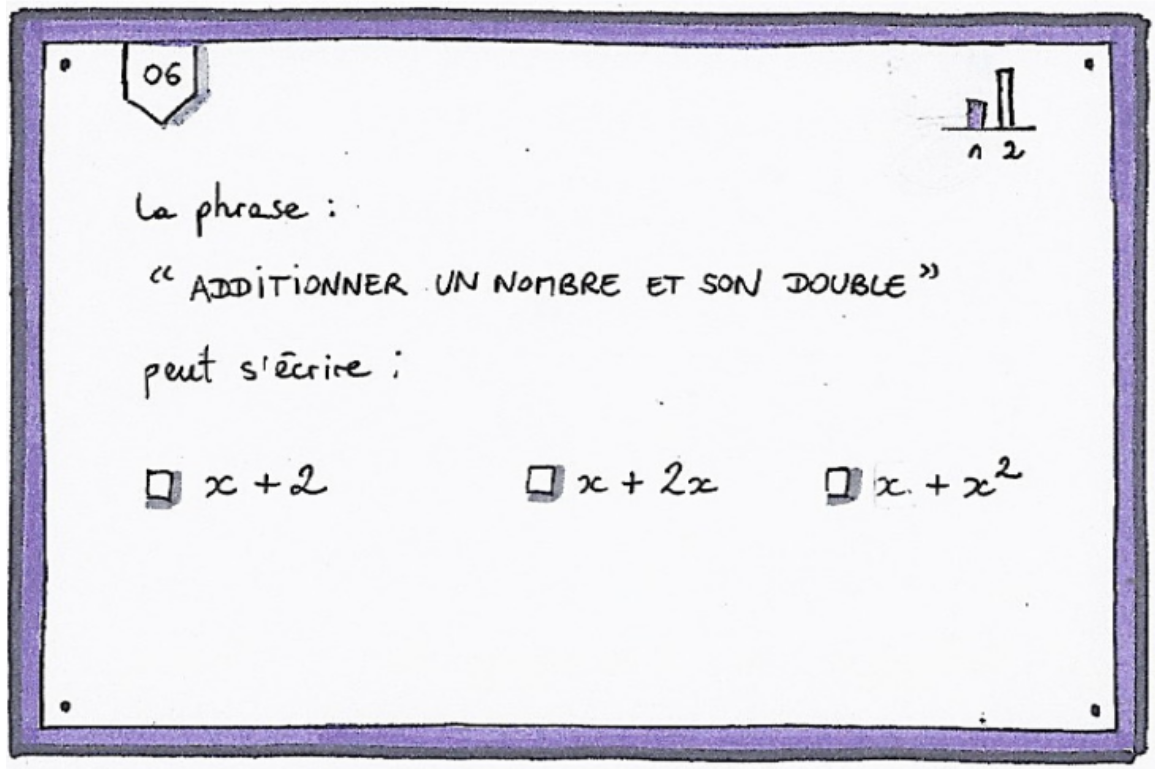
\includegraphics[width=0.95\linewidth]{Images/CalculLitteral4.png}
\end{center}
\end{exercice}

\begin{exercice}[Titre=En fonction de …]
    Exprimer en fonction du nombre $n$ :
    \begin{enumerate}
        \item Le triple de $n$.
        \item Le double de $n$.
        \item La moitié de $n$.
        \item Le périmètre d’un carré de côté $n$.
        \item L’aire d’un carré de côté $n$.
    \end{enumerate}
\end{exercice}

\begin{exercice}
    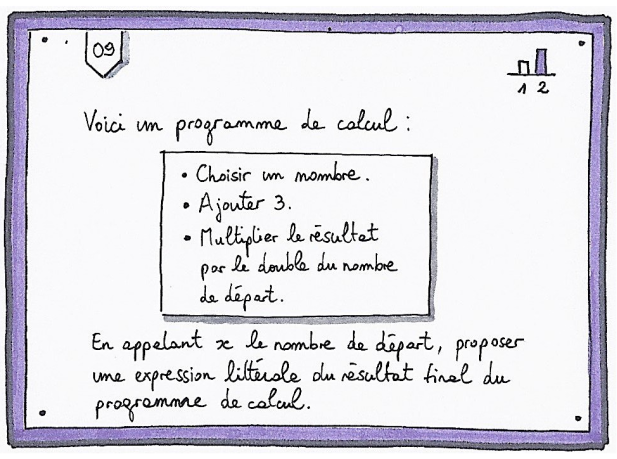
\includegraphics[width=\linewidth]{Images/CalculLitteral5.png}
\end{exercice}

\begin{exercice}
    Calcule la valeur de l’expression littérale 
    \[
    \textrm{A} = 5 n - 12
    \]
    lorsque :
    \begin{enumerate}
        \item $n=11$
        \item $n=4$
        \item $n=1$
        \item $n=2,4$
    \end{enumerate}
\end{exercice}

\begin{exercice}
    Calcule la valeur de l’expression littérale 
    \[
    \textrm{B} = \dfrac{x+1}{2} - 10
    \]
    lorsque :
    \begin{enumerate}
        \item $x=63$
        \item $x=40$
        \item $x=24$
        \item $x=7$
    \end{enumerate}

    Es-tu capable de trouver une valeur de $x$ pour laquelle $\textrm{B}=0$?
\end{exercice}

\end{Maquette}

\end{multicols}

\end{document}
